\chapter{Stability and Controllability}
\label{ch:Stability_and_Control}
In this chapter, the procedure used to ensure the stability and controllability of the \textit{Swing} design is described in detail. In \Cref{sec:Aileron_Sizing} the ailerons are sized, after which a hover control analysis has been performed in \Cref{sec:Hover_control}. From this, the CG is estimated in \Cref{sec:CG_loc} after which the tail is sized in \Cref{sec:Prel_tail}. The final configuration and the sizing of the horizontal and vertical tail sizing are done in \Cref{sec:tail_config}, \Cref{sec:Horizontal_tail} and \Cref{sec:Vertical_Tail_Sizing} respectively. After the final sizing, the dynamic stability during cruise is assessed in \Cref{sec:Dynamic_Stability_during_Cruise}, discussed in \Cref{sec:Results_Stability_and_Control} and verified in \Cref{sec:Stability_and_Control_V&V}.


\section{Preliminary Aileron Sizing}
\label{sec:Aileron_Sizing}
One of the first steps that can be taken to ensure that the design is controllable is to design the control surfaces in order to meet the rolling requirement.
According to CS 23 requirements, a General Aviation Aircraft should meet a \qty{60}{\degree} in 1.3 second rolling requirement \cite{easa_cs23_2020}.
However, since the aircraft is autonomous, flying quality level 3 can be used.
Additionally, from the mission profile of \Cref{ch:Mission_Profile} it becomes apparent that the \textit{Swing} will not have a conventional landing or take-off.
Therefore, the flight phase category B can be used~\cite{roll_requirement}.
This results in a roll rate requirement of \qty{60}{\degree} in 3.4 seconds.

It is important to consider that due to an increase in moment of inertia, which is caused by the battery placement as will be discussed in \Cref{sec:CG_loc}, the roll rate achieved will be smaller.
However, in the case of the preliminary sizing of the ailerons, the impact of the moment of inertia is not considered yet.
To be able to size the ailerons, the aileron roll rate equation should be considered first.
The roll rate is determined based on \Cref{eq:Aileron:Roll_rate}
\begin{equation}
    \label{eq:Aileron:Roll_rate}
    P=-\frac{C_{l_{\delta_{\text{a}}}}}{C_{l_P}} \delta a\left(\frac{2 V_\text{MC}}{b}\right)
\end{equation}

First, the minimum control speed used in the aileron sizing can be easily determined.
It can be assumed to maintain as much control as possible that the minimum control speed is equal to the stall speed \cite{mincontrolspeed}.
Based on this, the minimum control speed can be determined based on the stall speed equation:

\begin{equation}
    \label{eq:stall_speed}
    V_{\text{MC}} = \sqrt{\frac{2 W}{S \rho  C_{N_{\max}}}}
\end{equation}

The next parameter that can be determined empirically is the aileron deflection.
\Cref{eq;Aileron:delta_a} can be used to estimate the aileron deflection.
\begin{equation}
    \label{eq;Aileron:delta_a}
    \delta a=\frac{\delta a_{\text{up}}+\delta a_{\text{down}}}{2}
\end{equation}

Thus, it is important to determine the upward and downward assumed aileron deflection.
It can be assumed that a typical aileron has a maximum deflection of 30\degree.
Additionally, an efficiency of 75\% of the aileron is assumed \cite{gudmundsson2013general}.
Thus, the aileron deflection value can be assumed to be equal to $\delta_a= 22.5\degree$.
The next aspect that has to be determined is the airfoil used for the aileron sizing.
In the case of ailerons, typically used airfoils are symmetrical.
Therefore, the ailerons shall be sized taking a NACA0010 aileron airfoil into account.
This enables the determination of the aileron control derivative based on the following empirical equation~\cite{gudmundsson2013general}.

\begin{equation}
    \label{eq:Aileron:C_L_delta_alpha}
    C_{l_{\delta_{\text{a}}}}=\frac{2 c_{l_{\alpha}} \tau}{S_{\text{ref}} b} \int_{b_1}^{b_2} c(y) y d y
\end{equation}

The term $c_{l_{\alpha}}$ can be obtained from the airfoil characteristics, and it is equal to $c_{l_{\alpha}}=6.5 1/rad$.
Additionally, the aileron effectiveness parameter $\tau$ can be determined empirically, taking into account an aileron chord ratio of $c_f/c=0.25$.
This leads to an assumed value of $\tau = 0.45$, see \Cref{fig:Stab_and_control_tau}.

\begin{figure}[htpb]
    \centering
    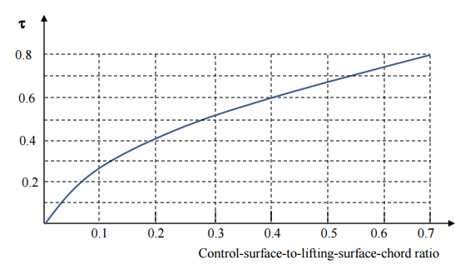
\includegraphics[width=0.6\textwidth]{figures/Stability & Controllability/tau}
    \caption{Aileron effectiveness as a function of the ratio of the
  aileron chord to the total airfoil chord~\cite{Aircraft_design:_a_systems_engineering_approach}}
    \label{fig:Stab_and_control_tau}
\end{figure}


Since the values of $S_\text{ref}$ and $b$ are known based on the wing planform, the last element that has to be calculated is the integral $\int_{b_1}^{b_2} c(y) y d y$.
To compute this integral, the chord as a function of span has to be determined.
This can be done based on \Cref{eq:Aileron:C(y)}:
\begin{equation}
    \label{eq:Aileron:C(y)}
    C(y) = C_{\text{r}} - \left( \frac{C_{\text{r}} - C_{\text{t}}}{b/2} \right) y
\end{equation}

It can be determined that $c(y)=1.42-0.122 y$. The only variable that has to be iterated is the aileron placement over the wing.
The last parameter that has to be determined is the roll damping derivative.
This can be done using \Cref{eq:Aileron:C_L_p}.
\begin{equation}
    \label{eq:Aileron:C_L_p}
    C_{l_p}=-\frac{4\left(c_{l_{\alpha}}+c_{d_0}\right)}{S_{\text{ref}} b^2} \int_0^{b/2} y^2 c(y) d y
\end{equation}\\
The parameters $c_{l_{\alpha}}$ and $c_{d_0}$ can be determined based on the NACA0010 airfoil used, whereas the integral can be computed based on the aforementioned chord equation.
Therefore, the roll damping derivative can be determined based on the position of the aileron on the wing.
It is important to note that the variables $b_1$ and $b_2$ represent the starting and end positions of the ailerons on the wingspan, and these variables are the variables that shall be sized for in this section. Before starting the iterations, a table with all the required constants for calculating the roll damping and the aileron roll rate, as well as their values, are presented in \Cref{tab:aileron_constants}.

\begin{table}[H]
    \centering
    \caption{Constants used in determining roll coefficients}
    \label{tab:aileron_constants}
    \begin{tabular}{ccccc}
        \toprule
        $c_{l_{\alpha}}$ & $\tau$ & $S_\text{ref}$ & b & $C_{d_0}$ \\
        \midrule
        \qty{6.5}{\per\radian} & 0.45 & \qty{14}{m^2} & \qty{14}{m} & 0.005 \\
        \bottomrule
    \end{tabular}
\end{table}

Now that all the constants have been determined to compute the roll rate in \Cref{eq:Aileron:Roll_rate}, the position of the aileron on the wing has to be iterated to reach the required roll rate.
The final aileron position and dimensions, as well as the achieved roll rate, shall be presented in \Cref{tab:aileron_design}, along with the required derivative parameters.
\begin{table}[H]
    \centering
    \caption{Aileron design values}
    \label{tab:aileron_design}
    \begin{tabular}{cccccccc}
        \toprule
        Airfoil & $b_1$ & $b_2$ & $\delta_a$ & $V_\text{MC}$ & $C_{l_{\delta_{\text{a}}}}$ & $C_{l_p}$ & P \\ \midrule
        NACA0010 & \qty{5.53}{m} & \qty{6.86}{m} & \qty{22.5}{\degree} & \qty{29.1}{\meter\per\second} & 0.43 & -0.85 & \qty{47.17}{\degree\per\second} \\ \bottomrule
    \end{tabular}
\end{table}


\section{Controllability in Hover Mode}
\label{sec:Hover_control}
The controllability during hover is analysed to increase the safety of the passengers and surroundings.
During hover, aerodynamic control surfaces will not be effective.
To analyse the vehicle’s controllability, the following method of \textcite{du2015controllability}.
The paper uses a linear dynamic model for the controllability with the assumption that rotorcraft, during hovering, ignores the aerodynamic damping and stiffness matrices, which results in \Cref{eq:dynhovermodel}. It utilises linearisation of the Newton Euler equations around hover conditions following from \textcite{pounds2002design}. 
\begin{equation}
\label{eq:dynhovermodel}
    \dot{\mathbf{x}} = A\mathbf{x} + B(\mathbf{F}-\mathbf{G}),\quad \text{with:}
\end{equation}

\noindent
\begin{minipage}[t]{0.45\textwidth}
\begin{align*}
\mathbf{x} &= \begin{bmatrix} h & \phi & \theta & \psi & v_h & p & q & r \end{bmatrix}^T \in \mathbb{R}^8 \\
\mathbf{F} &= \begin{bmatrix} T & L & M & N \end{bmatrix}^T \in \mathbb{R}^4 \\
\mathbf{G} &= \begin{bmatrix} m g & 0 & 0 & 0 \end{bmatrix}^T \in \mathbb{R}^4
\end{align*}
\end{minipage}
\hfill
\begin{minipage}[t]{0.45\textwidth}
\begin{align*}
{A} &= \begin{bmatrix} \mathbf{0}_{4 \times 4} & \mathbf{I}_4 \\ \mathbf{0}_{4 \times 4} & \mathbf{0}_{4 \times 4} \end{bmatrix} \in \mathbb{R}^{8 \times 8} \\
{B} &= \begin{bmatrix} \mathbf{0}_{4 \times 4} \\ \mathbf{J}_f^{-1} \end{bmatrix} \in \mathbb{R}^{8 \times 4} \\
{J}_f &= \operatorname{diag}\left(-m, J_x, J_y, J_z\right)
\end{align*}
\end{minipage}

The state vector, $\textbf{x}$, is dependent on the altitude $h$, the roll angle $\phi$, the pitch angle $\theta$,
the yaw angle $\psi$, vertical speed $v_h$, pitch rate $p$, roll rate $q$ and yaw rate $r$.
$\textbf{F}$ is the force vector, where $T$ is thrust, $L$ is roll torque, $M$ is the pitch torque and $N$ is yaw torque.
$\textbf{G}$ is the gravitational vector, $A$ is the state transition matrix, $B$ the control input matrix and $J_{f}$ the mass moment of inertia matrix. The input vector \textbf{u}, is defined as (\textbf{F} - \textbf{G}).

These input parameters for the ACAI are the locations of the rotors, the maximum thrust per engine, the total mass,
the rotor efficiency, the rotational direction of the propellers,
clockwise or anticlockwise, the efficiency parameter $\eta_{i}$,
ranging from zero to one, and the reactive torque coefficient $k_{\mu}$.
This coefficient is the ratio between the reactive torque and the lift.
This value was calculated to be equal to 0.1 complying with the literature~\cite{du2015controllability}.

The rotational direction configuration was set at PPNNPN, where P stands for clockwise rotation and N for anticlockwise rotation since this was stated to be most controllable in case of an engine failure~\cite{du2015controllability}.
To regard for engine failure, $\eta_{i}$ was set to zero for $i_{th}$ engine.
The final control effectiveness matrix $B_f$, which can be seen \Cref{eq:control_mat}.



\begin{equation}
\label{eq:control_mat}
B_f = \begin{bmatrix}
\eta_1 & \cdots & \eta_m \\
-\eta_1 r_1 \sin(\varphi_1) & \cdots & -\eta_m r_m \sin(\varphi_m) \\
\eta_1 r_1 \cos(\varphi_1) & \cdots & \eta_m r_m \cos(\varphi_m) \\
\eta_1 w_1 k_\mu & \cdots & \eta_m w_m k_\mu
\end{bmatrix}
\end{equation}

Where $r_{1}$ is the arm of from the CG to the propeller and $\phi_{m}$ the angle from the x-axis to the rotor, as can be seen in \Cref{fig:rotor_config}. It has to be noted that the CG in \Cref{fig:rotor_config} is preliminary and will be calculated later in \cref{sec:CG_loc}. \Cref{tab:engine_xy} shows the x- and y-locations of the engines measured from the nose of the vehicle. 

\begin{figure}[H]
    \centering
    \begin{minipage}{0.4\textwidth}
        \centering
        \captionof{table}{Coordinates of the engines measured from the nose of the vehicle}
        \label{tab:engine_xy}
        \begin{tabular}{l|c|c}
            \toprule
            Engines & x-coordinate [m] & y-coordinate [m] \\
            \midrule
            1,6 & 2.30 & $\pm$ 1.95 \\
            2,5 & 4.65 & $\pm$ 1.95 \\
            3,4 & 7.00 & $\pm$ 1.95 \\ 
            \bottomrule
        \end{tabular}
    \end{minipage}
    \hfill
    \begin{minipage}{0.4\textwidth}
        \centering
        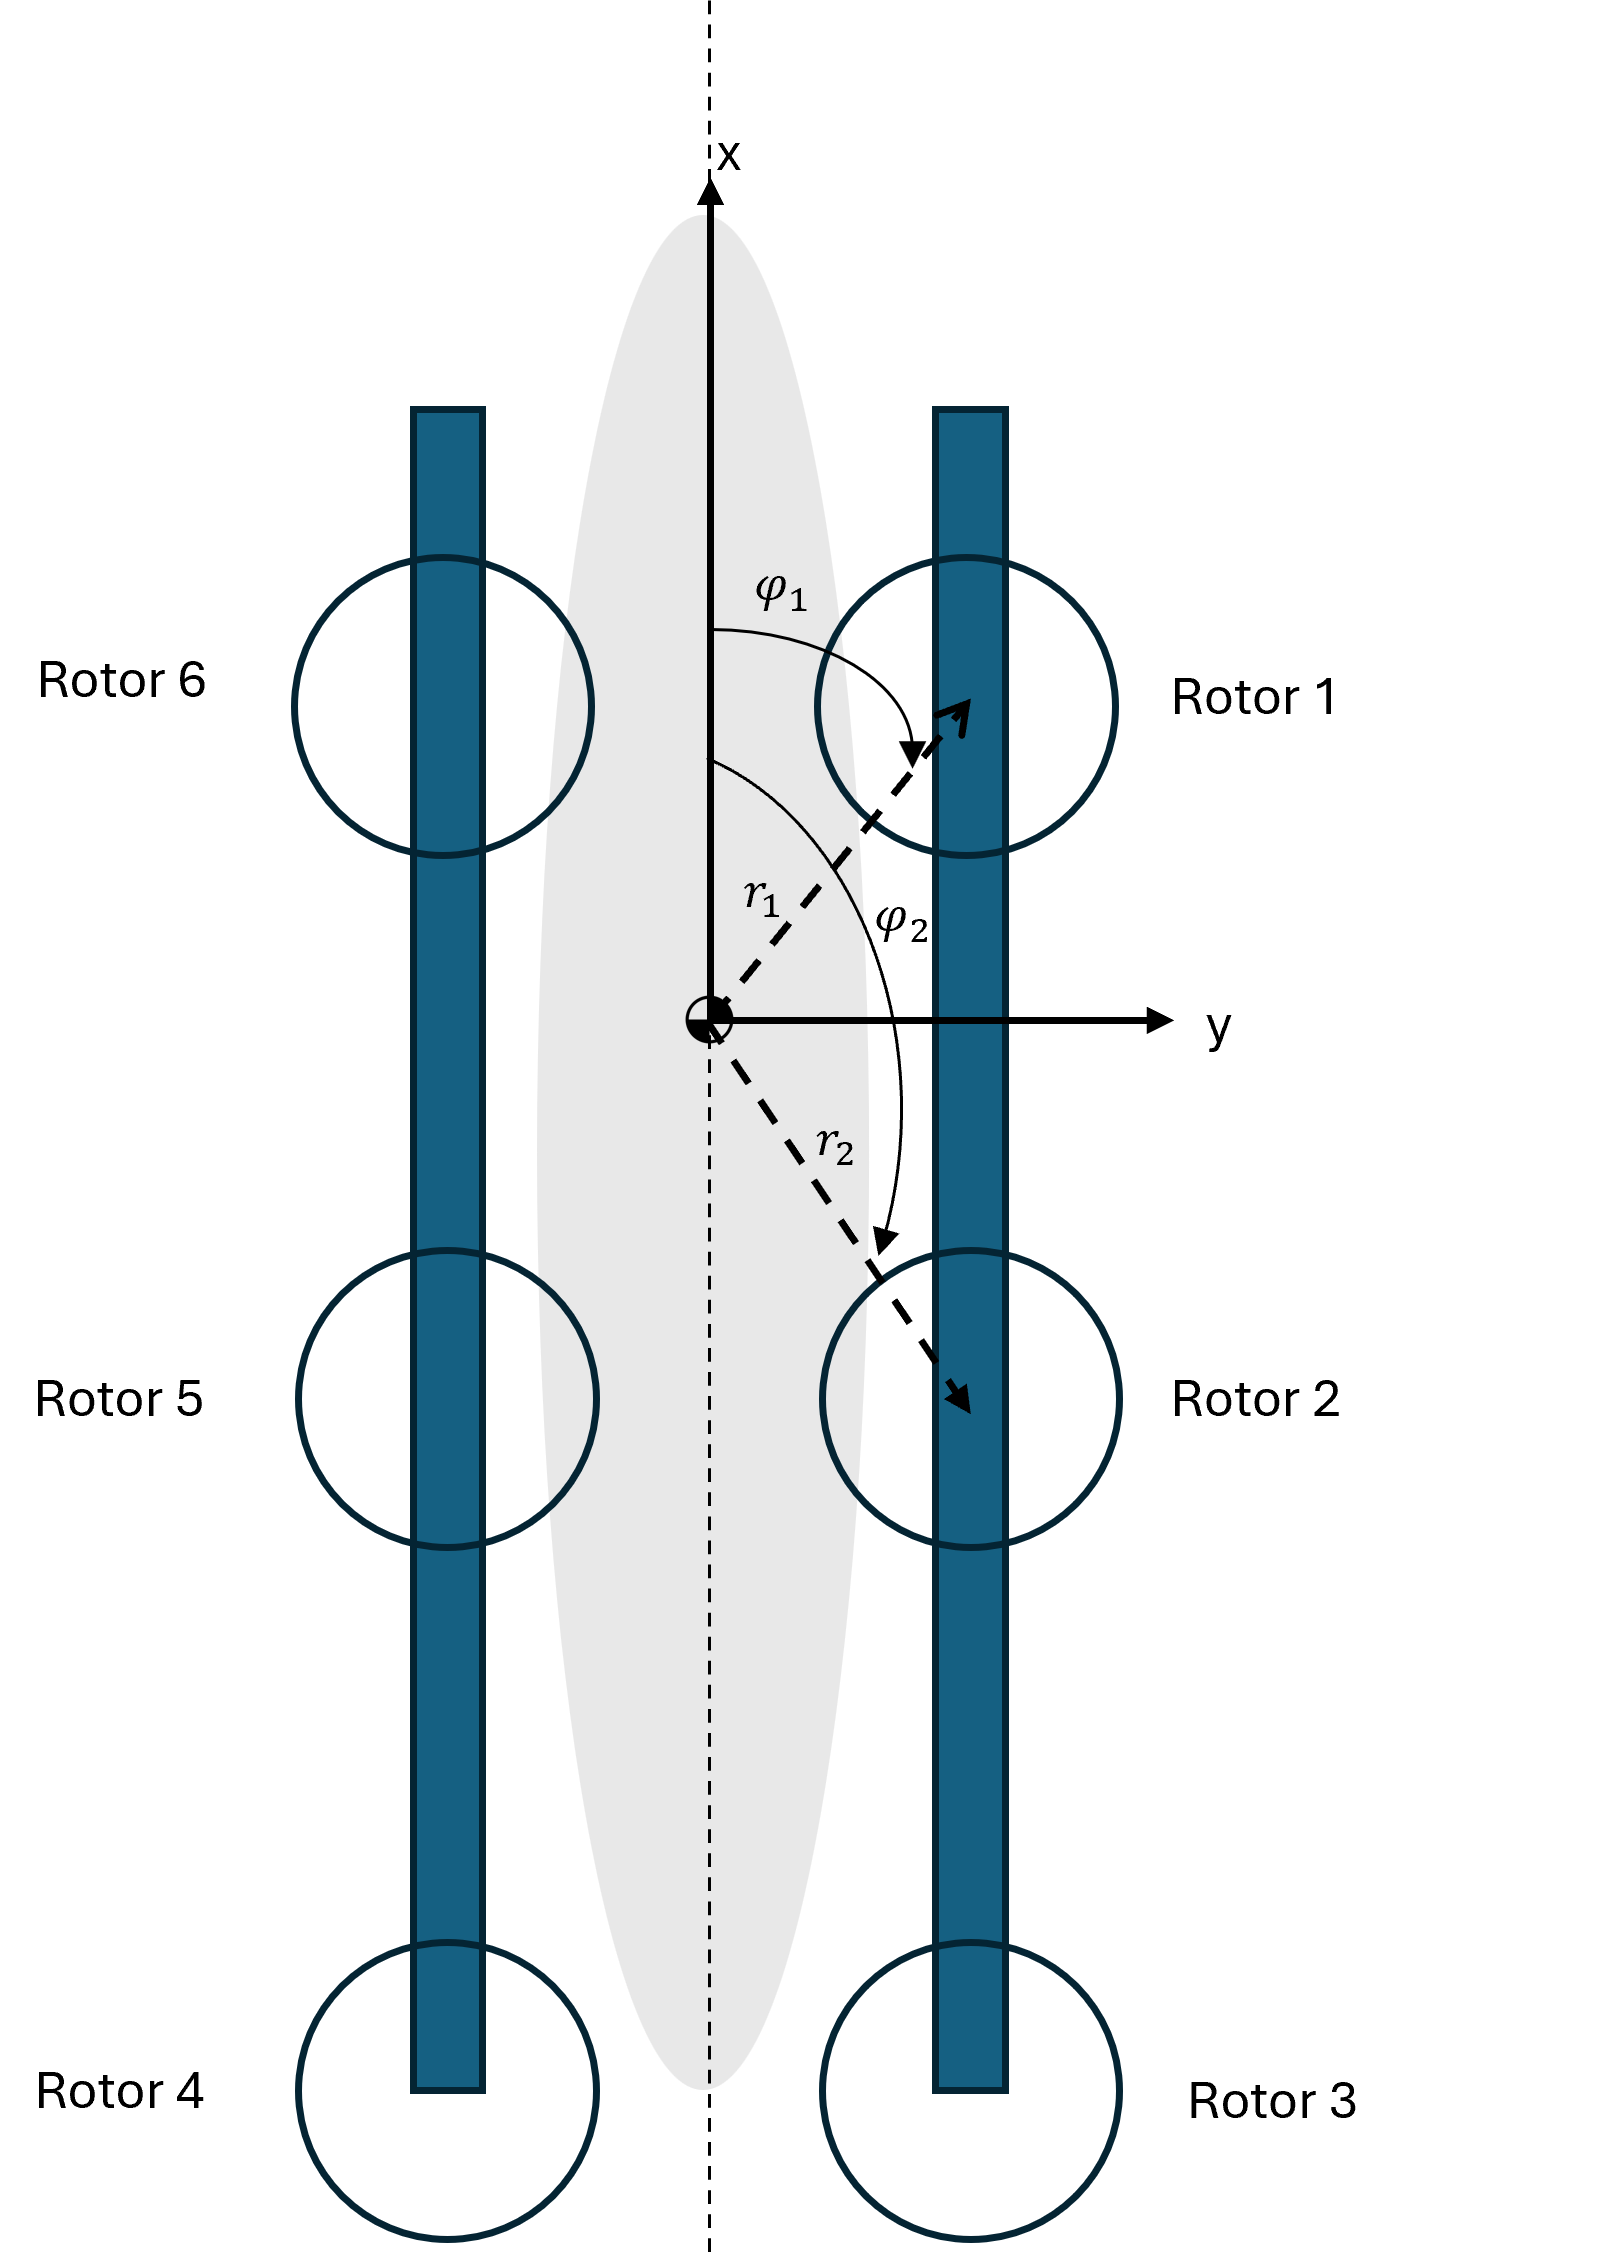
\includegraphics[width=\textwidth]{figures/Rotor config.png}
        \caption{Rotor configuration \textit{Swing}; Not to scale}
        \label{fig:rotor_config}
    \end{minipage}
\end{figure}



The total thrust/torque vector \textbf{F}  is dependent on the control effectiveness matrix and the trust per engine f, which is put into a vector and is constraint by \Cref{eq:space_f}

\begin{equation}
    \label{eq:space_f}
   \textbf{f} \in \textit{F} = \Pi^{m}_{i=1} [0,K_{i}] 
\end{equation}
Where $K_{i}$ is the maximum lift of \textit{i}th rotor in N. Using the geometry of the system and the mapping from the rotor lift, the system thrust/torque can be calculated as seen in \Cref{eq:tot_forcevect}
\begin{equation}
    \label{eq:tot_forcevect}
    \bm{F} = B_f \bm{f}
\end{equation}

From \Cref{eq:space_f} and \Cref{eq:tot_forcevect}, \textbf{F} is constrained by:

\begin{equation}
\label{eq:omegasubset}
\Omega = \{ \textbf{F} \mid \textbf{F} = \textbf{B$_f$}\textbf{f}, \textbf{f} \in \textit{F} \}
\end{equation}

Following from this, \textbf{u} is constrained by: 

\begin{equation}
    \label{eq:usubset}
    U = \{ \mathbf{u} \mid \mathbf{u} = \mathbf{F} - \mathbf{G}, \mathbf{F} \in \Omega \} 
\end{equation}

It can be seen from \Cref{eq:space_f,eq:omegasubset,eq:usubset}, \textit{F}, $\Omega$, and \textit{U} are convex and closed subsets. The purpose is to analyze the controllability by altering \textbf{u} under the constraint of subset \textit{U}. From this, a measure is defined as can be seen in \Cref{eq:ACAI_measure}.

\begin{equation}
\label{eq:ACAI_measure}
\rho(X, \partial \Omega) \triangleq 
\begin{cases}
    \min \{ \|X - F\| : X \in \Omega, F \in \partial \Omega \} & \text{if } X \in \Omega, F \in \partial \Omega \\
    -\min \{ \|X - F\| : X \in \Omega^C, F \in \partial \Omega \} & \text{if } X \in \Omega^C, F \in \partial \Omega
\end{cases}
\end{equation}
Where $\partial \Omega$ is the boundary of $\Omega$ and where $\Omega^c$ is the complementary set of $\Omega$. $\rho(X, \partial \Omega) $ is the radius of the maximum enclosed sphere in the control set $\Omega$, centred at \textbf{G}. This can be seen as the maximum control/torque produced in all directions and is therefore defined as the ACAI of the system \cite{du2015controllability}. It is based on the minimum Euclidean norm of the control force on the boundary of the control set $\Omega$. Moreover, the ACAI is independent on time.

The final ACAI was calculated using a Matlab Toolbox which was developed by \textcite{du2015controllability}.
 This toolbox calculated the ACAI, using the control effectiveness matrix, the minimum and maximum thrust setting per engine and the total thrust as input.
 The vehicle is deemed controllable if the ACAI is greater than zero.
 The CG (centre-of-gravity) was ranged between the most front and aft engine placement to analyse the controllability over the CG range,
which can be seen in \Cref{fig:Hov_cont}.
\begin{figure}[H]
    \centering
    \includegraphics[width=.6\textwidth]{figures/Stability & Controllability/Plot CGhover_all engine operative}
    \caption{ACAI value of the CG range at different thrust settings}
    \label{fig:Hov_cont}
\end{figure}
As can be seen in \Cref{fig:Hov_cont}, the vehicle is controllable if the CG is greater than \qty{3.4}{m} and smaller than \qty{5.8}{m} measured from the nose.
Therefore, the vehicle has to be sized to be within that CG range.
In case a safety factor of 1.1 is applied, the CG is stable from \qty{3.67}{m}.

One of the requirements is that the aircraft has to be operative if one engine fails during flight.
This was analysed by setting $\eta_{i}$ to zero for the designated engine.
This was performed for all engines separately, and in all configurations, the aircraft was deemed controllable.
However, the maximum thrust per engine had to be increased, and thus, violated the noise requirement.
However, if an engine fails, this is considered an emergency and therefore violating the requirement is allowed.


\section{CG-Location Determination}
\label{sec:CG_loc}
The first step in the determination of the stability and controllability of the vehicle during operation is the determination of the location of the centre-of-gravity.
This shall be done in two steps.
Firstly, the CG-location is determined empirically based on the design of the fuselage and wings. Afterwards, a loading diagram is created to ensure that the CG is within the desired range.
\subsection{Class I CG Determination}
\label{subsec:Class_I_CG_determination}
First and foremost, it can be considered that the wing placement is performed based on the fuselage shape as well as the ground footprint requirement.
Additionally, since the difference in required CG for cruise as well as for hovering is rather significant.
As shall be described during this chapter, it was intended that the wing has a large CG excursion during transition to obtain the required CG shift.
Based on these considerations as well as on the shape of the fuselage, the leading edge of the wing was placed \qty{1.6}{m} from the front of the fuselage.

Another aspect that influences the CG shift is the position of the batteries.
To ensure the required CG excursion and to save as much space as possible, the batteries are placed in the nacelles of the engines situated in the wing.
The engines situated closest to the tip shall carry most of the battery weight to ensure the required CG shift.
However, this decision has a significant drawback with regard to the rolling requirement.
This is caused by the increase in moment of inertia which limits the dynamic characteristics of the design.
The reduced rolling performance shall be discussed in more detail in \Cref{sec:Dynamic_Stability_during_Cruise}

After establishing these preliminary aspects, it is important to discuss how the centre of gravity is determined for both phases.
To compute the CG excursion, \Cref{eq:CG_excursion} shall be used, where $i$ represents a particular weight component.
Those weight components have to be established.
\begin{equation}
    \label{eq:CG_excursion}
    X_{CG}=\frac{\sum M_i \cdot X_i}{\sum M_i}
\end{equation}

Another aspect that has to be taken into account for the determination of the CG, is that in cruise four different CGs must be considered:
\begin{itemize}
    \item Operating Empty Weight (OEW) CG
    \item OEW + luggage
    \item OEW + luggage + back-row passengers
    \item OEW + full payload
\end{itemize}

A table with all the CG components,
their masses and the locations of the components, as well as the final CG values for the cruise configuration, shall be provided in \Cref{tab:CG_cruise}.

\begin{table}[H]
    \centering
\caption{Cruise CG Range}
    \label{tab:CG_cruise}
\begin{tabular}{l|S[table-format=1.2]S[table-format=4]}
\toprule
\textbf{Component}                 & \textbf{Position on $x$-axis } {[}m{]} & \textbf{Mass } {[}kg{]} \\
\midrule
Fuselage, fixed equipment & 2.40                       & 284           \\
Wing                      & 2.17                       & 349           \\
Empennage                 & 7.20                       & 27            \\
Engine nacelle 1          & 2.25                       & 61            \\
Engine nacelle 2          & 2.39                       & 61            \\
Engine nacelle 3          & 2.54                       & 61            \\
Front seat                & 1.65                       & 160           \\
Back seat                 & 2.50                       & 160           \\
Luggage                   & 3.00                       & 80            \\
Battery                   & 2.31                       & 400           \\
\midrule
\textit{Fuselage Group}   & \textit{2.50}              & \textit{711}  \\
\textit{Wing Group}       & \textit{2.28}              & \textit{933}  \\
\bfemph{Total}            & \bfemph{2.37}              & \bfemph{1644} \\
    \bottomrule
\end{tabular}
\end{table}

Now that the cruise configuration centre of gravity is determined, the next step is to determine the CG during the VTOL phase.
It is important to ensure that in hovering, the CG is situated in between the values determined with the use of the ACAI tool as described in \Cref{sec:Hover_control}.

To determine the CG during hover, it is crucial to understand which components have different CGs in hovering compared to the cruising phase.
The shift in CG is mostly caused by the change in the position of the wing with respect to the longitudinal position.
Thus, the centre of gravity of the wing, the engines as well as the batteries change while the other components remain fixed.
Based on these considerations, the following centre of gravity is obtained for hover configuration in \Cref{tab:CG_hover}.

\begin{table}[H]
    \centering
    \caption{Hovering CG Range}
    \label{tab:CG_hover}
    \begin{tabular}{l|S[table-format=1.2]S[table-format=4]}
        \toprule
        \textbf{Component}                 & \textbf{Position on $x$-axis } {[}m{]} & \textbf{Mass } {[}kg{]} \\
        \midrule
        Fuselage, fixed equipment & 2.40                       & 284           \\
        Wing                      & 2.96                       & 349           \\
        Empennage                 & 7.20                       & 27            \\
        Engine nacelle 1          & 2.30                       & 61            \\
        Engine nacelle 2          & 4.65                       & 61            \\
        Engine nacelle 3          & 6.99                       & 61            \\
        Front seat                & 1.65                       & 160           \\
        Back seat                 & 2.50                       & 160           \\
        Luggage                   & 3.00                       & 80            \\
        Battery                   & 5.97                       & 400           \\
        \midrule
        \textit{Fuselage Group}   & \textit{2.50}              & \textit{711}  \\
        \textit{Wing Group}       & \textit{4.58}              & \textit{933}  \\
        \bfemph{Total}            & \bfemph{3.68}              & \bfemph{1644} \\
        \bottomrule
    \end{tabular}
\end{table}

Initially, the CG during hover was situated outside the ACAI requirement.
However, to tackle this issue, the battery mass was increased leading to a further backward shift of the CG
Therefore, with a battery mass increase to 400 kg, the final CG position during hover is situated within the controllability limits of the hovering phase.

\subsection{Loading Diagram}
 The next crucial step is to establish whether the design is stable and controllable during the cruise phase.
 To achieve this step, it is crucial to size the aircraft tail as well as establish its configuration.
 This step has to be performed after a more detailed centre-of-gravity analysis is performed.
 To be able to find out a more detailed CG excursion, a loading diagram analysis should be performed.

 In the loading diagram, the loading of the cargo and the passengers is taken into account.
 Before delving into the CG determination, it is important to note that the vehicle shall be restricted to load back to front due to the fact that the backward seats are only accessible when the front seats are folded.
 To determine the CG for every new loading case, the following \Cref{eq:CG_loading} shall be employed.

 \begin{equation}
     \label{eq:CG_loading}
    X_{\text{CG}_\text{new}} = \frac{W_\text{old}\cdot X_{\text{CG}_\text{old}} + W_\text{item}\cdot X_{\text{CG}_\text{item}}}{W_\text{old} + W_\text{item}}
 \end{equation}

 In this equation, the starting weight is considered to be the operating empty weight as determined previously.
 Based on these assumptions, the following loading diagram is obtained for the SWING design in \Cref{fig:load_diagram}.

 \begin{figure}[htpb]
     \centering
     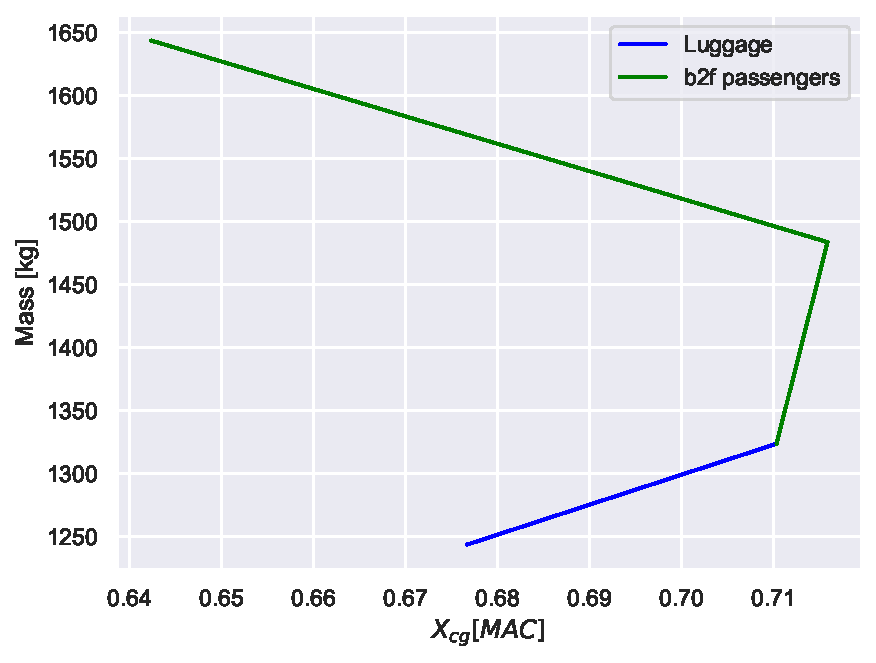
\includegraphics[scale=0.7]{figures/Stability & Controllability/loading diagram}
     \caption{SWING loading diagram}
     \label{fig:load_diagram}
 \end{figure}

 To determine the tail size, the most aft CG location has to be considered as well as the CG range.
 From the diagram it can be seen that the values for the most aft and most forward CG are the following:
$X_\text{aftCG}=\qty{2.46}{m}$ and $X_\text{fwCG}= \qty{2.37}{m}$.
 Thus, the CG range is situated between 64 and 72\% of the mean aerodynamic chord.
 The next step that has to be taken to ensure stability and controllability is determining the tail size.
\section{Preliminary Estimation of Tail Size} \label{sec:Prel_tail}
 To be able to properly determine the size of the tail and enable proper iterations, it is important to first size the tail based on previous aircraft designs.
This ensures that the preliminary estimations are feasible and provide valuable insight with regard to the sizing of the tail.
This step is crucial; since the size of the tail is very restricted, due to the ground footprint restrictions
Thus, with the preliminary estimations of the tail size, the location and dimensions, as well as the tail configuration, can be determined.
Thus, to determine the preliminary size of the tail, it is crucial to assume the tail volume coefficients.
These coefficients can be assumed based on literature and previous designs.
According to \citeauthor{Roskam_Part_2}~\cite{Roskam_Part_2}, $\overline{V_h}=0.9$.
\citeauthor{scholz2021empennage}~\cite{scholz2021empennage} states that $\overline{V_v}=0.0601$.

After considering the tail volume coefficients, the horizontal tail surface area can be computed using the following equation:
\begin{equation}
    \overline{V_h}=\frac{(X_h-X_\text{aftCG})S_h}{S\overline{c}}
\end{equation}
where $X_h$ is the spanwise location of the mean aerodynamic chord of the horizontal tail, $X_\text{aftCG}$ is the spanwise location of the most aft centre of gravity of the aircraft, $S_h$ is the surface area of the horizontal tail, $S$ is the surface area of the wing, and $\overline{c}$ is the mean aerodynamic chord of the wing.
The value of $S_h$ is then calculated assuming the value of $X_h$ as determined in the CG location calculations.
Additionally, the vertical tail surface area can be determined by use of a similar equation:
\begin{equation}
    \overline{V_v}=\frac{(X_v-X_\text{aftCG})S_v}{Sb}
\end{equation} 
Now that the surface areas are determined and fixed, the tail planform can be properly determined.
In order to achieve this goal, the aspect ratios of the tails have to be considered.
However, if a typical value of the aspect ratio of the vertical tail of 2 is assumed \cite{HAW_9} and a taper ratio of 0.4 is also considered, the span of the vertical tail can be calculated to have a value of 2.6 meters.
Taking this value into account, the span would exceed the vertical ground footprint requirement of 2 meters, and as such, a conventional tail configuration would be unfeasible.
This requires analysis of different concepts which shall be performed in the next section.

\section{Tail Configuration and Planform }
\label{sec:tail_config}
First and foremost, it is important to note that the design shall make use of a high-wing configuration.
This, in turn, implies that there would be a significant wake on the horizontal stabiliser of a conventional tail.
Thus, only two different tail configurations would be feasible, the T-tail and the V-tail.
However, due to the limited vertical footprint requirement, the T-tail configuration is impossible to design for. Thus, the only feasible design option is an inverted V-tail.

To size the inverted V-tail, several steps have to be determined, based on the fact that the horizontal contribution and vertical contribution of the tail are integrated into one single angled surface.
The first step that has to be taken to size the surface is to determine the angle at which the inverted V-tail is situated with respect to the horizontal plane.
This can be done on the basis of \Cref{eq:V_tail_angle}~\cite{HAW_9}:
\begin{equation}
    \label{eq:V_tail_angle}
    \nu = \arctan\frac{S_v}{S_h}
\end{equation}
with the values of $S_v$ and $S_h$ determined in \Cref{sec:Prel_tail}.
While the analytical method suggests that the final area of the design shall be equal to $S_{tail}=\sqrt{S_v^2+S_h^2}$ due to inefficiencies of the V-tail design, it has to be assumed that $S_{tail}=S_v+S_h$.
Now that the total tail surface has been calculated, the new vertical and horizontal components should be redetermined to enable sizing of the wing planform:
\begin{equation}
    S_{v_\text{new}=S_\text{tail}*\sin(\nu)},\quad S_{h_\text{new}=S_\text{tail}*\cos(\nu)}
\end{equation}

After having determined the surface areas of each component, it is important to be able to determine the geometrical parameters of the tail itself.
Since it is clear that the horizontal footprint is limiting, the chord of the design shall be determined based on the horizontal tail, and then the other properties of the vertical tail shall be determined.

Based on the literature, vertical tails usually have an aspect ratio situated between 1 and 2~\cite{Roskam_Part_2}.
To reduce the chord size of the tail, an aspect ratio of two was assumed for the initial sizing.
It is known that $A=b^2/S$, which implies that the vertical \enquote{wingspan} of the tail can be determined.
Thus, the space occupied by the tail on the vertical plane can be determined by using the following equation:
\begin{equation}
    b_v= \sqrt{A_v \cdot S_{v_\text{new}}}
\end{equation}

To determine the space occupied in the vertical plane, the total span should now be halved.
The division by 2 is caused by the fact that the V-tail is composed of two elements, the total span on the horizontal plane represents the sum of the contribution of each of the two components.
This leads to a vertical contribution which is double compared to the vertical space taken.
Thus, $h_\text{tail}=b_v/2$.
Performing preliminary calculations, it can be seen that the tail height is lower than 2 meters, so it can be ensured that the tail fits within footprint requirements.

After the span is computed, the root chord of the aircraft can be determined from which the horizontal component span and aspect ratio can be determined.
The horizontal components as well as the total tail span can be computed using the following formulas:

\begin{minipage}{0.45\linewidth}
    \begin{equation}
    c_r=\frac{2\cdot S_V}{{1+\lambda} \cdot b_v}
\end{equation}
\end{minipage}
~
\begin{minipage}{0.45\linewidth}
    \begin{equation}
    b_h=\frac{2\cdot S_h}{{1+\lambda} \cdot c_r}
\end{equation}
\end{minipage}

\begin{minipage}{0.45\linewidth}
\begin{equation}
    A_h=\frac{b_h^2}{S_h}
\end{equation}
\end{minipage}
~
\begin{minipage}{0.45\linewidth}
\begin{equation}
    b = \sqrt{b_h^2+b_v^2}
\end{equation}
\end{minipage}

Thus, taking into account that $c_t = \lambda \cdot c_r$, all the tail parameters are computed and the preliminary tail planform can be finalised.

\section{Horizontal Tail Sizing}
\label{sec:Horizontal_tail}
Now that the tail has finally been preliminarily sized, it is crucial that the tail planform is designed to ensure that it provides both enough stability and controllability on the horizontal plane.
This step is taken by use of a scissor plot, whose creation method shall be expanded upon in this section.

\subsection{Stability Requirement}\label{subsec:Stability_horiz}
When it comes to the longitudinal stability requirement,
the primary stability condition is
that the centre of gravity of the aircraft is located ahead of the stick-fixed neutral point of the design.
Thus, the first curve that is used in configuring the scissor plot is the stick-fixed stability curve, given in \Cref{Eq:stability_curve}.
\begin{equation}
    \label{Eq:stability_curve}
    \frac{S_h}{S} = \frac{1}{\frac{C_{L_{\alpha_h}}}{C_{L_{\alpha_{A-h}}}}\left(1 - \frac{d\epsilon}{d\alpha}\right)\frac{l_h}{\bar{c}}\left(\frac{V_h}{V}\right)^2}\bar{x}_{c.g.}-\frac{\bar{x}_\text{ac}-0.05}{\frac{C_{L_{\alpha_h}}}{C_{L_{\alpha_{A-h}}}}\left(1 - \frac{d\epsilon}{d\alpha}\right)\frac{l_h}{\bar{c}}\left(\frac{V_h}{V}\right)^2}
\end{equation} 
In this equation, the second term represents a safety margin of 5\% that is assumed to ensure that the design is not susceptible to stability issues.
It is clear that in order to properly size the curve, several parameters such as $C_{L_{\alpha_h}}$ are yet undefined.
Thus, first and foremost the values of $\bar{x}_\text{ac}$, $C_{L_{\alpha_h}}$, $C_{L_{\alpha_A-h}}$, $d\epsilon/d\alpha$ and $V_h/V$ have to be determined.

The first parameter that can be analysed is the $V_h/V$ ratio.
This represents the velocity of the airstream that reaches the horizontal tail with respect to the wing.
Due to the position of the wing (high wing), as well as the inverted position of the tail, the interference of the wing on the tail airflow is considered to be minimal.
Thus, the tail is assumed to be similar to a fin-mounted stabiliser in the velocity ratio aspect, and thus the ratio is assumed to have a value of $\frac{V_h}{V}^2=0.95$ \cite{Seville}.

On the basis of the tail position, the downwash is also estimated to be 0 since the interference is minimal.
Thus $\frac{d\epsilon}{d\alpha} = 0$.
The next parameter that needs to be determined is $C_{L_{\alpha_h}}$, the lift rate coefficient of the horizontal tail.
This can be calculated using \Cref{eq_claplhah}\cite{DATCOM}

\begin{equation}
    \label{eq_claplhah}
    C_{L_{\alpha_h}} = \frac{2\pi A_h}{2+\sqrt{4+\left(\frac{A_h\beta}{\eta}\right)^2\left(1+\frac{tan^2(\Lambda_{0.5C_h})}{\beta^2}\right)}}
\end{equation}

With $\beta = \sqrt{1-M^2}$, $M = V/a$ and finally, $a = \sqrt{TR\gamma}$, using ISA conditions to obtain the temperature based on the cruise altitude.
Additionally, the lift coefficient of the tailless aircraft has to be considered $C_{L_{\alpha_{A-h}}}$.
This parameter can also be determined on the basis of an empirical equation~\cite{torenbeek_1982}:
\begin{equation}
    \label{eq:C_l_alpha_A-h}
    C_{L_{\alpha_{A-h}}} = C_{L_{\alpha_w}}\left(1+2.15\frac{b_f}{b}\right)\frac{S_\text{net}}{S}+\frac{\pi}{2}\frac{b_f^2}{S}
\end{equation}

In this equation, the parameters $b_f$ and $S_\text{net}$ represent the width of the fuselage and the net wing surface area (the section inside the fuselage is removed).

Lastly, the aerodynamic centre of the aircraft can also be computed through the calculation of the influences of the nacelles, the wing and the fuselage.
The contribution of the wing and the fuselage shall be determined with the use of \Cref{eq:x_ac_wf}.
\begin{equation}
    \label{eq:x_ac_wf}
    \left(\frac{x_\text{ac}}{\bar{c}}\right)_{wf} = \left(\frac{x_\text{ac}}{\bar{c}}\right)_w-\frac{1.8}{C_{L_{\alpha_{A-h}}}}\frac{b_fh_fl_{fn}}{s\bar{c}}+\frac{0.273}{1+\lambda}\frac{b_fc_f\left(b-b_f\right)}{\bar{c}^2\left(b+2.15b_f\right)}tan\left(\Lambda_{1/4}\right)
\end{equation}

The first term of \Cref{eq:x_ac_wf} is the contribution of the wing, which is found experimentally\cite{torenbeek_1982}.
The second term is the forward shift of the aerodynamic centre due to the fuselage nose’s contribution to lift.
Lastly, the third term is the aft shift of the aerodynamic centre due to the loss of lift at the intersection of the fuselage and wing.
The contribution of the nacelles is now calculated in \Cref{eq:ac_nacelles}~\cite{torenbeek_1982}.

\begin{equation}
    \label{eq:ac_nacelles}
    \Delta_n\frac{x_\text{ac}}{\bar{c}} = \sum{k_n}\frac{b_n^2l_n}{s\bar{c}\left(C_{L_{\alpha}}\right)_{A-h}}
\end{equation}

Where $k_n \approx -4$ for nacelles mounted in front of the leading edge of the wing.
It is important to note that in \Cref{eq:ac_nacelles} $C_{L_{\alpha}}$ should be in [\unit{rad^{-1}}] and $l_n$ is considered positive when the nacelle is located in front of the 1/4 MAC.

Now that all the data is obtained, the stability curve can be plotted.

\subsection{Controllability Requirement} \label{subsec:Control_horiz}
As it is clear from the stability equation, moving the CG forward enables a more stable aircraft design.
However, when taking controllability into account, it is more relevant to move the CG aft,
since a forward CG implies an increase in pitching up and a pitching down moment required.
Thus, when it comes to the controllability requirement, the tail size with respect to the wing size as a function of CG can be described based on the following equation:

\begin{equation}
    \label{Eq:Controllability_curve}
    \frac{S_h}{S} = \frac{1}{\frac{C_{L_{h}}}{C_{L_{A-h}}}\frac{l_h}{\bar{c}}\left(\frac{V_h}{V}\right)^2}\bar{x}_{c.g.}+\frac{\frac{C_{m_\text{ac}}}{C_{L_{A-h}}}-\bar{x}_\text{ac}}{\frac{C_{L_{h}}}{C_{L_{A-h}}}\frac{l_h}{\bar{c}}\left(\frac{V_h}{V}\right)^2}
\end{equation}

Based on this equation, several parameters have to be analysed.
First and foremost, the lift coefficient of the horizontal tail used on the aircraft $C_{L_{h}}$ can be derived using analytical relations. This is dependent on the type of tail that is used, whether fixed, adjustable or full moving.
To improve the controllability of the design, a full moving tail is chosen; therefore, $C_{L_h} = -0.35\cdot A_h^{1/3}$.

Another parameter that has to be sized is the pitching moment coefficient at the aerodynamic centre of the aircraft, which can be found by calculating the moment contributions of the fuselage, wing and engine nacelles~\cite{torenbeek_1982}:

\begin{equation}
    \label{eq:C_m_ac}
    C_{m_\text{ac}} = C_{m_{ac,w}} + \Delta_{fus} C_{m_\text{ac}} + 2\cdot \Delta_{nac} C_{m_\text{ac}}
\end{equation}

It is important to note that the design shall not undergo typical take-off and landing procedures.
Therefore, there is no need to make use of flaps to increase the lift coefficient of the aircraft.
This implies that the contribution of the flaps to the moment can be ignored.
The contribution of the wing and fuselage are found using empirical equations~\cite{torenbeek_1982}:
\begin{equation}
    C_{m_{ac,w}} = C_{m_{0,\text{airfoil}}}\left(A\cos^2(\Lambda)/\left(A+2\cos(\Lambda)\right)\right)
\end{equation}
\begin{equation}
    \Delta_{fus} C_{m_\text{ac}} = -1.8\left(1-\frac{2.5b_f}{l_f}\right)\frac{\pi b_fh_fl_f}{4S\bar{c}}\frac{C_{L_0}}{C_{L_{\alpha,(A-h)}}}
\end{equation}

Thus, to be able to correctly determine the wing contribution to the pitching moment, the airfoil contribution has to be inferred first.
This can be done considering the assumed sweep and aspect ratio and taking into account the pitching moment of the chosen Eppler 423 airfoil. Additionally, to determine the total fuselage contribution, the lift at zero angle of attack has to be determined.
Lastly, the nacelle pitching moment increment should be analysed as well. This can be calculated using the following equation \cite{Etkinflight}:
\begin{equation}
    \Delta_{nac} C_{m_\text{ac}}= C_{m_{\text{ac}_{0}}} + C_{L_w} \cdot (-\Delta_n\frac{x_\text{ac}}{\bar{c}})
\end{equation}

Where the nacelle contribution has already been calculated in \Cref{eq:ac_nacelles}.
Thus, to determine the nacelle pitching moment, the wing lift has to be determined as well as the zero-lift nacelle pitching moment.
The lift of the aircraft wing can be retrieved based on the design of the wing and has a value of $C_L=0.73$.
The zero-lift nacelle pitching moment can be estimated by assuming that the wing has no fillet and considering the fact that the aircraft has a high wing configuration $C_{m_{\text{ac}_{0}}}=0.004$~\cite{Etkinflight}.

\subsection{Scissor Plot}
Considering the parameters explained in \Cref{subsec:Control_horiz,subsec:Stability_horiz}, the scissor plot can be obtained in \Cref{fig:scissor_plot}:
\begin{figure}[H]
    \centering
    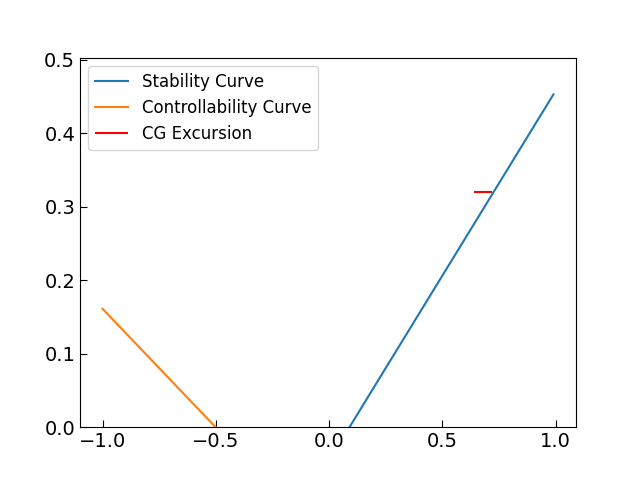
\includegraphics[scale=0.7]{figures/Scissor}
    \caption{Scissor plot}
    \label{fig:scissor_plot}
\end{figure}
As it can be noticed, the horizontal tail ratio has to have a minimum value of around $\frac{S_h}{S}=0.32$ to meet the stability requirement.
Additionally, it is noticeable that the controllability requirement is not constraining.
This is reasonable since the tail is sized for cruise conditions, not landing conditions since landings shall be performed in VTOL configuration.
Thus, a final horizontal tail surface ratio of 0.32 shall be taken into account when sizing the final design.
Therefore, the final horizontal tail size can be assumed to have a value of \qty{4.48}{\m^2}.
\section{Vertical Tail Sizing}
\label{sec:Vertical_Tail_Sizing}

The vertical tail will be sized on two criteria, namely, the weathervane stability and the engine inoperative.
The most limiting criteria will determine the size of the vertical tail.

\subsection{Vertical Tail Sizing Stability Requirement}
\label{subsec:Vertical_Tail_Sizing_Stability_Requirement}

To achieve stability, the stability derivative $C_{N_{\beta}}$ (the weathervane stability) needs to be positive.
To achieve sufficient static directional stability $C_{N_{\beta}}$ should be greater or equal than $0.0571 \frac{1}{rad} $\cite{Roskam_Part_2}. $C_{N_{\beta}}$ can be calculated using \Cref{eq:C_N_beta_total}.

\begin{equation}
    \label{eq:C_N_beta_total}
    C_{N_{\beta}} = \left(C_{N_{\beta}}\right)_{f} + \left(C_{N_{\beta}}\right)_{w} + \left(C_{N_{\beta}}\right)_{v}
\end{equation}

Where $f$ is the fuselage contribution, $v$ is the contribution of the vertical tail and $w$ is the contribution of the wing.
The contribution of the wing is neglected because \enquote*{The contribution to $C_{N_\beta}$ of a wing without sweep is very small}~\cite{FD_LectureNotes}.
The vertical tail and fuselage contributions can be found using \Cref{eq:C_N_beta_fuselage,eq:C_N_beta_tail}

\begin{equation}
    \label{eq:C_N_beta_fuselage}
    \left(C_{N_{\beta}}\right)_{f} = -\frac{2 \nu}{S b}
\end{equation}

As can be seen in \Cref{eq:C_N_beta_fuselage} \cite{M&AE5070Notes} the fuselage has a destabilising effect on the directional stability of the aircraft.
$\nu$ is the volume of the equivalent fuselage, $S$ is the wing area and $b$ is the wing span.


\begin{equation}
    \label{eq:C_N_beta_tail}
    \left(C_{N_{\beta}}\right)_{v} = -C_{Y_{v_\alpha}} \cdot\left(1-\frac{d \sigma}{d \beta}\right) \cdot\left(\frac{V_v}{V}\right)^2 \cdot \frac{S_v l_v}{S b}
\end{equation}
In \Cref{eq:C_N_beta_tail} \cite{FD_LectureNotes} $C_{Y_{v_\alpha}}$ is the derivative of the side force of the vertical tail with respect to the angle of the vertical tail. $\frac{d \sigma}{d \beta}$ is the side wash, which because of simplicity is assumed to be 0. $\frac{V_v}{V}$ is the ratio between the free stream velocity and the velocity at the vertical tail, this ratio is assumed to be 1.
The side force generated due to the vertical tail ($C_{Y_{v_\alpha}}$) is the negative of the lift coefficient of the vertical tail ($C_L{_{v_\alpha}}$). $l_{v}$ is the moment arm of the vertical tail.
Rewriting \Cref{eq:C_N_beta_total,eq:C_N_beta_tail} results in the required vertical tail surface.

\begin{equation}
    \label{eq:Tail_area_stability}
    \left(\frac{S_v}{S}\right)_\text{required} =\frac{C_{n_\beta}-\left(C_{n_\beta}\right)_{f}}{C_{L_{v_\alpha}}} \cdot \frac{b}{l_v}
\end{equation}



\subsection{Vertical Tail Sizing Control Requirement}
\label{subsec:Vertical_Tail_Sizing_Control_Requirement}
Another important aspect to consider that is crucial in achieving a complete design, is the controllability requirement of the vertical tail.
This requirement is determined by the all-engine inoperative requirement, where all engines fail on one side of the aircraft.
The aircraft is required to maintain equilibrium with the help of rudder deflection in the case of a multi-engine failure~\cite{easa_cs23_2020}.

Thus, the moments generated by the active engines compared to the failed engines have to be computed first, as well as the moment generated by the drag of the inoperative engines.
The following formulas are given for calculating each engine’s moment contribution with respect to the symmetry plane due to the thrust of the active engine as well as the drag of the inoperative engine:

\begin{minipage}{0.45\textwidth}
    \begin{equation}
    N_E=T_{\max} \cdot y_E
\end{equation}
\end{minipage}
~
\begin{minipage}{0.45\textwidth}
   \begin{equation}
    \label{eq:N_D}
    N_D=0.75\cdot N_E
\end{equation} 
\end{minipage}

\Cref{eq:N_D} is estimated based on the fact that the design shall make use of fixed-pitch propellers.
In these equations, $N_E$ represents the moment caused by the active engine, $y_E$ is the placement of the engine on the span, whereas $N_D$ is the moment generated by the drag of the inoperative engine.

To be able to size the vertical stabiliser, the condition is that all engines on one side of the aircraft fail.
Thus, all moment contributions of all engines have to be summed up: $N_{E_\text{tot}}=\sum N_{E_{i}}$ and $N_{D_\text{tot}}=\sum N_{D_{i}}$.
To correct the engine thrust asymmetry generated sideslip, it is assumed that only the rudder surface is used as correction of the moment.
The moment caused by the rudder can be calculated based on DATCOM \cite{DATCOM}:
\begin{equation}
    N_V=\frac{1}{2}\rho V_\text{MC}^2\cdot \delta_f \cdot \frac{C_{l,\delta}}{C_{l,\delta_\text{theory}}} \cdot C_{l,\delta_\text{theory}} \cdot K' \cdot K_{\Lambda} \cdot S_v \cdot l_v
\end{equation}

In this equation, $V_\text{MC}$ represents the minimum control speed and is equal to the same speed as used to size the ailerons in \Cref{sec:Aileron_Sizing}.
Thus, if the design is sized for equilibrium such that $N_{E_\text{tot}}+N_{D_\text{tot}}= N_V$, the tail size can be determined with the following formula:

\begin{equation} \label{eq:S_V_control2}
    S_V=\frac{N_{E_\text{tot}}+N_{D_\text{tot}}}{\frac{1}{2}\rho V_\text{MC}^2\cdot \delta_f \cdot \frac{C_{l,\delta}}{C_{l,\delta_\text{theory}}} \cdot C_{l,\delta_\text{theory}} \cdot K' \cdot K_{\Lambda} \cdot l_v}
\end{equation}

Thus, to be able to come up with the final tail design, several parameters such as K' and $K_{\Lambda}$ have to be defined.
The definition of these parameters shall be provided in \Cref{tab:vert_control}.
Afterwards, the value for each of the parameters shall be explained in more detail.

\begin{table}[H]
    \centering
    \caption{Values required to determine the vertical tail size for engine inoperative}
    \label{tab:vert_control}
    \resizebox{\textwidth}{!}{
    \begin{tabular}{ccccccccccc}
        \toprule
        $N_E$ & $N_D$ & $\rho$ & $V_\text{MC}$ & $C_{l,\delta_\text{theory}}$ & $\frac{C_{l,\delta}}{C_{l,\delta_\text{theory}}}$ & K' & $K_{\Lambda}$ & $\delta_f$ & $l_v$ & $S_v$ \\ \midrule
        \qty{146}{kNm} & \qty{109}{kNm} & \qty{1.17}{\kg\per\m^3} & \qty{29.1}{m/s} & 3.6 & 0.74 & 0.65 & 0.92 & \qty{25}{\degree} & \qty{4.74}{m} & \qty{2.73}{m^2} \\ \bottomrule
    \end{tabular}
    }
\end{table}

Now, the values computed for $N_E$ and $N_D$
are based solely on the thrust determined in \Cref{ch:Propulsion} as well as the locations of the engine.
The density is based on the mission profile as described in \Cref{ch:Mission_Profile}, whereas the minimum control speed is determined in \Cref{sec:Aileron_Sizing}.
Lastly, the moment arm of the tail is determined based on the CG position of the tail.

The parameters that have to be determined empirically are the other parameters.
First and foremost, the theoretical flap efficiency has to be determined, as well as the ratio between the flap efficiency and the theoretical one ($C_{l,\delta_\text{theory}}$ and $\frac{C_{l,\delta}}{C_{l,\delta_\text{theory}}}$). This can be done assuming that the rudder shall employ a NACA0012 flap as well as a 0.2 flap chord-to-empennage chord ratio.
\Cref{fig:flap_efficiency,fig:K',fig:sweep_corr} shall be used for the determination of these parameters \cite{HAW_11}.

\begin{minipage}{0.45\linewidth}
\begin{figure}[H]
    \centering
    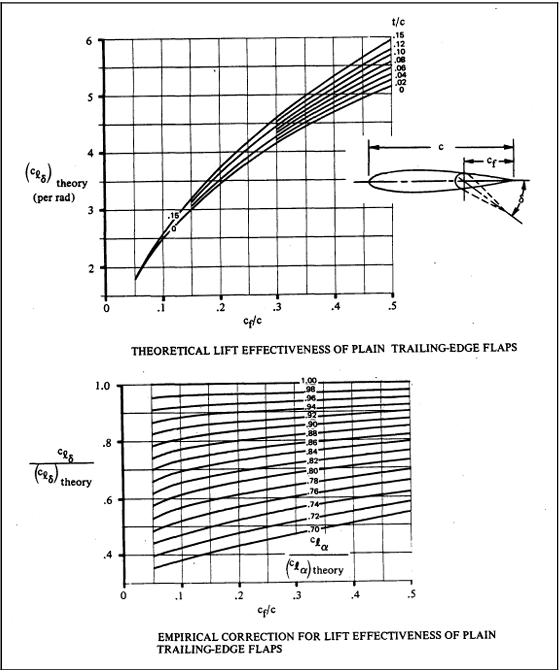
\includegraphics[scale=0.5]{figures/Flap efficiency}
    \caption{Lift effectiveness of plain trailing-edge flaps}
    \label{fig:flap_efficiency}
\end{figure}
\end{minipage}
\hfill
\begin{minipage}{0.45\linewidth}
\begin{figure}[H]
    \centering
    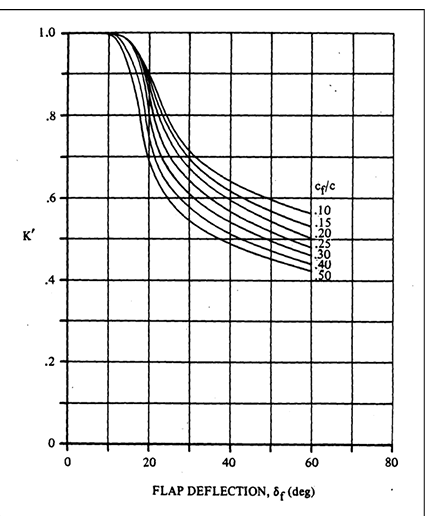
\includegraphics[scale=0.65]{figures/Flap deflection}
    \caption{Empirical correction for non-linear effects at bigger flap angles}
    \label{fig:K'}
\end{figure}
\end{minipage}

The next parameters that should be determined are K' and $K_\Lambda$.
K' can be determined considering the 0.2 assumed chord ratio, based on empirical data plots.
Additionally, a flap deflection of $\delta_f = \qty{25}{\degree}$ based on typical rudder deflections is assumed \cite{HAW_11}.
This yields a K' value of 0.65 as per \Cref{fig:K'}:



Lastly, the sweep correction factor $K_\Lambda$ can also be sized empirically.
First of all, the empennage sweep has to be assumed.
The empennage sweep must be equal to 0 to ensure that the tail is situated within the ground footprint requirement.
Thus, $K_\Lambda=0.65$ based \Cref{fig:sweep_corr}~\cite{HAW_8}:

\begin{figure}[H]
    \centering
    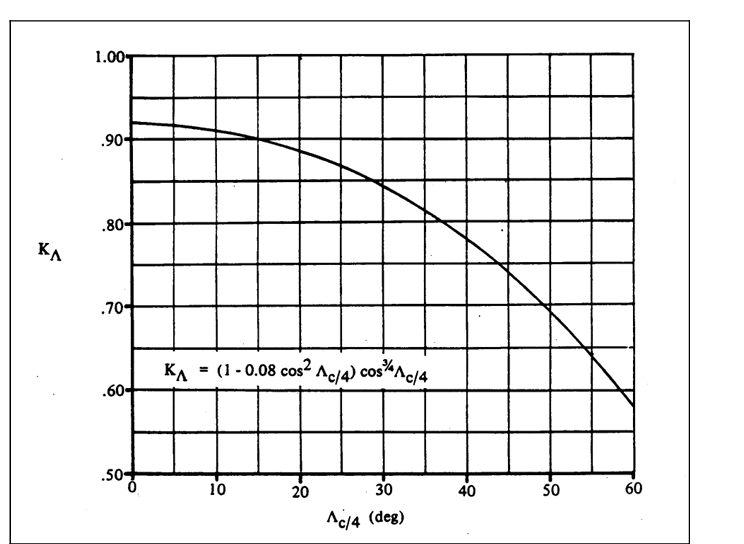
\includegraphics[scale=0.5]{figures/Sweep correction}
    \caption{Sweep correction factor}
    \label{fig:sweep_corr}
\end{figure}

With all these empirical factors determined, the final minimum vertical tail size can be computed.
This yields a value of \qty{2.73}{\m^2}.

%\subsection{Discrepancies between preliminary sizing and stability and control requirement}
\section{Dynamic Stability during Cruise}
\label{sec:Dynamic_Stability_during_Cruise}

To analyse the dynamic stability of the \textit{Swing} during cruise, a state space model is created.
Both for the longitudinal and lateral cases the model is created.

\subsection{Longitudinal Stability}
\label{subsec:Longitudinal_Stability}

The equations of motion for the longitudinal stability can be found in \Cref{eq:dynamic:EOM:Long}~\cite{FD_LectureNotes}.
The stability parameters used in the equations of motion are gathered from the AeroSandbox tool \cite{aerosandbox}.
This is explained in more detail in \Cref{sec:AeroBuildup}, and the stability coefficients can be found in \Cref{tab:stability_coefficients}.
The eigenvalues ($\lambda = \xi_c + \eta_c$ $j$) of the $4\times4$ matrix determine the stability of the \textit{Swing} eVTOL. The real part of all the eigenvalues need to be negative to insure dynamic stability.
The eigenvalues can be determined by replacing the $D_c$ by $\lambda$ and then solving for $\lambda$.
The eigenvalues can be found in \Cref{fig:Eigenvalues_Long}, it can be seen that all the real part of each eigenvalue is negative.

\begin{equation}
    \label{eq:dynamic:EOM:Long}
     {\left[\begin{array}{cccc}
    C_{X_u}-2 \mu_c D_c & C_{X_\alpha} & C_{Z_0} & C_{X_q} \\
    C_{Z_u} & C_{Z_\alpha}+\left(C_{Z_{\dot{\alpha}}}-2 \mu_c\right) D_c & -C_{X_0} & C_{Z_q}+2 \mu_c \\
    0 & 0 & -D_c & 1 \\
    C_{m_u} & C_{m_\alpha}+C_{m_{\dot{\alpha}}} D_c & 0 & C_{m_q}-2 \mu_c K_Y^2 D_c
    \end{array}\right]\left[\begin{array}{c}
    \hat{u} \\
    \alpha \\
    \theta \\
    \frac{q \bar{c}}{V}
    \end{array}\right]} \\
     =\left[\begin{array}{c}
    -C_{X_{\delta_e}} \\
    -C_{Z_{\delta_e}} \\
    0 \\
    -C_{m_{\delta_e}}
    \end{array}\right] \delta_e
\end{equation}

\begin{figure}[h]
    \centering
    \begin{subfigure}[b]{0.49\textwidth}
        
\includegraphics[width=1\linewidth]{figures/Stability & Controllability/Eigen_Values_Long}
    \caption{Eigenvalues in longitudinal motion}
    \label{fig:Eigenvalues_Long}
    \end{subfigure}
    ~
    \begin{subfigure}[b]{0.49\textwidth}
        
\includegraphics[width=\linewidth]{figures/Stability & Controllability/Eigen_Values_Lat}
    \caption{Eigenvalues in lateral motion}
    \label{fig:Eigenvalues_Lat}
    \end{subfigure}
    \caption{Eigenvalues dynamic model}
    \label{fig:Eigenvalues_both}
\end{figure}

With the eigenvalues, one can calculate the time to half the amplitude, the period, the damping ratio and the natural frequency. \Cref{eq:dynamic:symT0.5,eq:dynamic:symP,eq:dynamic:symZeta} can be used to calculate these, in \Cref{tab:Characteristic_values_of_eigenmotions} these characteristics can be found.
For the longitudinal stability, the two eigenmodes are the \textit{Short Period} and \textit{Phugoid}.

\noindent\begin{minipage}{0.33\linewidth}
\begin{equation}
    T_{\frac{1}{2}} = \frac{ln \frac{1}{2}}{\xi_c} \frac{\bar{c}}{V}
    \label{eq:dynamic:symT0.5}
\end{equation}
\end{minipage}
~
\begin{minipage}{.33\linewidth}
\begin{equation}
    P = \frac{2\pi}{\eta_c} \frac{\bar{c}}{V}
    \label{eq:dynamic:symP}
\end{equation}    
\end{minipage}
~
\begin{minipage}{.33\linewidth}
\begin{equation}
    \zeta = \frac{-\xi_c}{\sqrt{\xi_c^2 + \eta_c^2}}
    \label{eq:dynamic:symZeta}
\end{equation}    
\end{minipage}

\begin{table}[h]
\centering
\caption{Characteristic values of eigenmotions}
\label{tab:Characteristic_values_of_eigenmotions}
\sisetup{table-format=+2.3, round-mode=figures, round-precision=3}
\begin{tabular}{l|SSS}
\toprule
\textbf{Eigenmotion}     & \textbf{Period [\unit{s}]} & \textbf{Damping Ratio [\unit{-}]} & \textbf{Amplitude Halving Time [\unit{s}]} \\ \midrule
Short Period    & 4.209513133    & 0.153038192           & 2.998688776                    \\
Phugoid         & 23.53423569    & 0.031567748           & 82.20260722                    \\
Dutch Roll      & 9.962827219    & 0.303351156           & 3.452392922                    \\
Roll Subsidence & {-}            & 1                     & 0.294445148                    \\
Spiral          & {-}            & -1                    & -0.860502916  \\
\bottomrule
\end{tabular}
\end{table}


\subsection{Lateral Stability}
\label{subsec:Lateral_Stability}

The Lateral stability has been performed similarly to the longitudinal stability.
The equations of motion can be found in \Cref{eq:dynamic:EOM:Lat}~\cite{FD_LectureNotes}.
In \Cref{fig:Eigenvalues_Lat} the eigenvalues of the lateral motion can be found, in contrast to the eigenvalues of the longitudinal motion; not all the eigenvalues are negative.
The real part of the eigenvalue that is corespondent with the spiral eigenmode is positive; however, there are many aircraft that are spirally unstable. \Cref{tab:Characteristic_values_of_eigenmotions} shows that the amplitude halving time of the spiral is negative, it thus is the time to double the amplitude.
This doubling tim is small, so an iteration is recommended.
The spiral stability can be improved
by lowering the vertical tail area and thus the $C_{n_{\beta}}$, or by changing the dihedral of the wing
to increase the magnitude of the $C_{l_{\beta}}$.
From \Cref{tab:Characteristic_values_of_eigenmotions} it can also be seen that there is no period for both the \textit{Roll Subsidence} and the \textit{Spiral}.
Because the eigenvalues corresponding to those eigenmodes do not have an imaginary part, therefore the period is infinite, and the magnitude of the damping ratio will be 1.

\begin{equation}
\label{eq:dynamic:EOM:Lat}
\begin{aligned}
& {\left[\begin{array}{cccc}
C_{Y_\beta}+\left(C_{Y_{\dot{\beta}}}-2 \mu_b\right) D_b & C_L & C_{Y_p} & C_{Y_r}-4 \mu_b \\
0 & -\frac{1}{2} D_b & 1 & 0 \\
C_{\ell_\beta} & 0 & C_{\ell_p}-4 \mu_b K_X^2 D_b & C_{\ell_r}+4 \mu_b K_{X Z} D_b \\
C_{n_\beta}+C_{n_{\dot{\beta}}} D_b & 0 & C_{n_p}+4 \mu_b K_{X Z} D_b & C_{n_r}-4 \mu_b K_Z^2 D_b
\end{array}\right]\left[\begin{array}{c}
\beta \\
\varphi \\
\frac{p b}{2 V} \\
\frac{r b}{2 V}
\end{array}\right]=} \\
&=\left[\begin{array}{cc}
-C_{Y_{\delta_a}} & -C_{Y_{\delta_r}} \\
0 & 0 \\
-C_{\ell_{\delta_a}} & -C_{\ell_{\delta_r}} \\
-C_{n_{\delta_a}} & -C_{n_{\delta_r}}
\end{array}\right]\left[\begin{array}{c}
\delta_a \\
\delta_r
\end{array}\right]
\end{aligned}
\end{equation}


As mentioned in \Cref{subsec:Class_I_CG_determination} the ailerons that have been sized in \Cref{sec:Aileron_Sizing} will most likely not be able to achieve sufficient roll performance due to the large mass moment of inertia about the x-axis.
To investigate the implications of this, the lateral dynamic is used, and an aileron deflection ($\delta_{\text{a}}$) of $22.5 \deg$ is used.
To further reduce the effect of the mass moment of inertia on the roll performance, the ailerons are now placed on the entire span of the wing to improve the roll performance.
\Cref{fig:roll_vs_time} shows the results; it can be seen that in 6 seconds the \textit{Swing} can roll \qty{60}{\degree}.
The roll rate can be found in \Cref{fig:rollrate_vs_time}.
It should be noted that this is at cruise speed and with the maximum aileron deflection, this is the best case for roll performance.
Therefore, it can be concluded that the roll requirement of \qty{60}{\degree} in 3.4 seconds is not achieved.
Therefore, this requirement should be critically analysed in further iterations of the design.
Moreover, the roll requirement itself should be critically analysed because the roll requirement is based on small light aircraft as there is currently no roll requirement for (e)VTOLs.
The current roll performance is showcased in \Cref{fig:roll3D}



\begin{figure}[h]
    \centering
    \begin{subfigure}[b]{0.49\textwidth}
        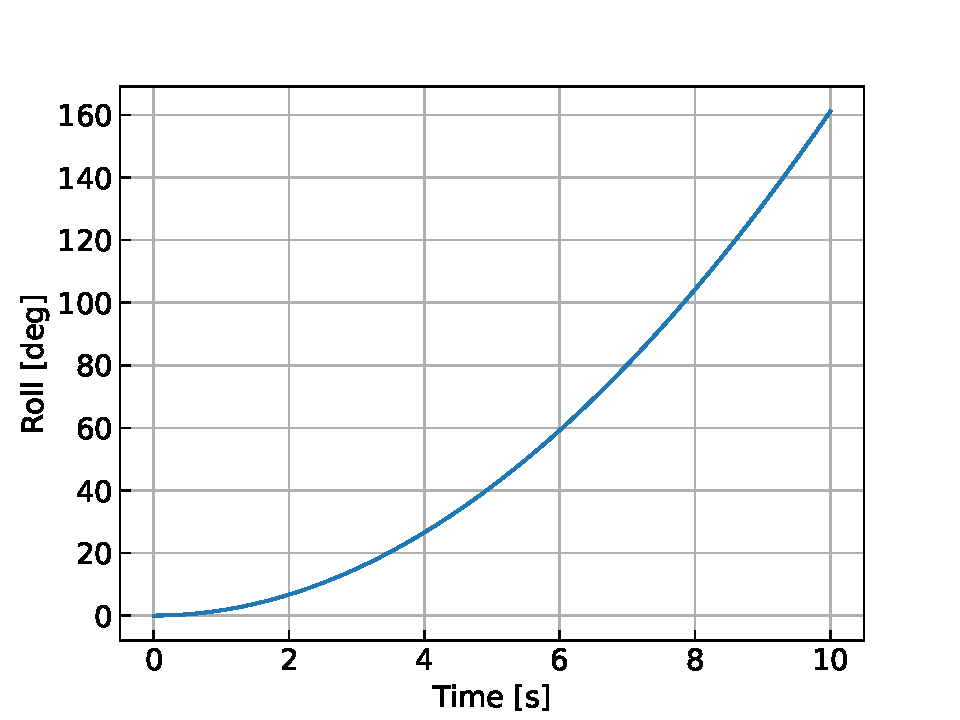
\includegraphics[width=1\linewidth]{figures/Stability & Controllability/Roll_Lat}
    \caption{Roll versus time at $V_{\text{Cruise}}$ with $\delta_{\text{a}} = 22.5 \deg$ }
    \label{fig:roll_vs_time}
    \end{subfigure}
    ~
    \begin{subfigure}[b]{0.49\textwidth}
        
\includegraphics[width=\linewidth]{figures/Stability & Controllability/Roll_rate_Lat}
    \caption{Roll rate versus time at $V_{\text{Cruise}}$ with $\delta_{\text{a}} = 22.5 \deg$ }
    \label{fig:rollrate_vs_time}
    \end{subfigure}
    \caption{Roll performance analysis}
    \label{fig:Roll_Performance_Analysis}
\end{figure}

\begin{figure}[htpb]
    \centering
    
\includegraphics[width=0.7\textwidth]{figures/Stability & Controllability/roll3D}
    \caption{Roll performance for a duration of \qty{6}{\s} with $\delta_{\text{a}} = 22.5 \deg$ at $V_{\text{cruise}}$visualised in 3D space. Aircraft scale is 5-to-1 for visibility}
    \label{fig:roll3D}
\end{figure}


\section{Results and Discussion}
\label{sec:Results_Stability_and_Control}
Now that both the horizontal and the vertical stabiliser sizing methods have been described, the final tail configuration can be established.
The most important tail parameters shall be described below for both the class I and the class II sizing in \Cref{tab:Tail_Parameters}.
\begin{table}[H]
    \centering
    \caption{Tail Parameters}
    \label{tab:Tail_Parameters}
    \sisetup{table-format=1.2}
    \resizebox{\textwidth}{!}{
    \begin{tabular}{l|SSSSSSSS[table-format=2.2]SSS}
        \toprule
        & $S_h [\unit{m^2}]$ & $S_v [\unit{m^2}]$ & $S_\text{tail} [\unit{m^2}]$ & $A_v [\unit{-}]$ & $A_h [\unit{-}]$ & $\Lambda_h [\unit{-}]$ & $\Lambda_v [\unit{-}]$ & $\nu$ [\unit{-}] & $b_\text{tail} [\unit{m}]$ & $c_r [\unit{m}]$ & $c_t [\unit{m}]$ \\ \midrule
        Preliminary & 2.82 & 2.48 & 5.30 & 2.00 & 2.27 & 0.40 & 0.40 & 41.38 & 4.00 & 1.89 & 0.76 \\
        Class II & 4.48 & 2.73 & 7.21 & 1.52 & 2.50 & 0.40 & 0.40 & 31.36 & 4.59 & 2.24 & 0.90 \\ \bottomrule
    \end{tabular}
    }
\end{table}

\section{Verification \& Validation}
\label{sec:Stability_and_Control_V&V}
An important aspect that has to be performed to ensure the correctness of the results is the assess the quality of the code.
This can be done based on verification and validation procedures.

First and foremost, several unit tests have been conceptualised in order to assess the correctness of the Python code utilised in sizing the tail.
Thus, unit tests were performed on the scissor plot Python code to determine whether the outputs correspond to expected values.

\subsubsection{Scissor Plot Unit Test}
Several tests were conceptualised in order to ensure the correctness of the computed parameters.
Thus, the following unit tests were performed:
\begin{table}[H]
\centering
\caption{Scissor plot unit tests}
\begin{tabular}{p{1.5cm} p{2.2cm} p{2.5cm} p{2cm} p{2cm} p{2cm} p{1.5cm}}
\hline
Test ID & Technique                                                           & Description                                                                         & Justification                                                      & Tolerance & Result & Confidence \\ \hline
SCI-1   & Manual Calculation  & Test correctness of parameter calculation & Easy to perform, accurate & 10\%       & Pass   & High       \\
SCI-2   & Visual inspection of plot & Test final plot correctness                                                         & Easy to perform, & N/A       & Pass   & High      
\end{tabular}
\end{table}

\subsubsection{Dynamic Model Unit Test}
Another aspect that is crucial to the stability and controllability of the design is the dynamic model.
Therefore, it is important to come up with unit tests for the dynamic model as well.
The following unit tests were performed on the dynamic model:

\begin{table}[H]
\centering
\caption{Dynamic model unit test}
\label{tab:unit_tests_module_1}
\begin{tabular}{p{1.5cm} p{2.2cm} p{2.5cm} p{2cm} p{2cm} p{2cm} p{1.5cm}}
\toprule
Test ID & Description  & Technique & Justification & Tolerance & Result & Confidence \\ \midrule
DYN-1   & \raggedright Check of Data input shape  & Print shape of loaded data  & Easy, Accurate       & N/A       & \raggedright Retrieves data in correct shape & High
\\
DYN-2 & \raggedright Check of Data Unit  & \raggedright Visual inspection of the dataset  & Easy, Accurate       & N/A       & \raggedright Units are as expected & High
\\
DYN-3 & \raggedright Check output correctness  & \raggedright Test whether Cessna 172 aircraft is stable according to model  & Verify result feasibility       & N/A       & \raggedright Aircraft is stable & High \\
DYN-4 &\raggedright Symmetric Matrix Check & \raggedright Creation of matrix & \raggedright Verify that matrix is correctly constructed   &  N/A       & \raggedright Matrix matches expected outcome & High
\\
DYN-5   & \raggedright Asymmetric matrix check  & Creation of matrix & \raggedright Verify that matrix is correctly constructed  &  N/A      & \raggedright Matrix matches expected outcome & High\\
\bottomrule
\end{tabular}
\end{table}

Next, validation of the final design values should be performed.
Since there is a lack of availability in data for eVTOL designs, validating the final tail sizes is challenging.
However, to determine whether the results are feasible or not, a comparison between final design parameters and class I values can be performed.
A short discussion of the discrepancies between the values is thus in order.

It can be seen that the horizontal tail is significantly larger in the class II estimation.
However, the reason for this issue is that the CG is positioned very aft compared to the mean aerodynamic chord of the wing compared to a typical design.
Additionally, the vertical tail size is high for the class II estimation as well since all engines are considered inoperative in the sizing of the tail.

However, a more detailed analysis of the competitor tail sizes should be performed whenever more data becomes available.
It is clear from the final design values that the vertical tail is oversized, and this should be taken into account further down the road during the next design phases.

\section{Further Iterations and Recommendation}
\label{sec:Further_Iterations_and_Recommendation}

As it can be seen, the current design of the aircraft has severe spiral instability, with a doubling time of 0.8 seconds.
This is considerably below the requirement of a minimum doubling time of 5 seconds \cite{cook2012flight}.
Therefore, since spiral instability is caused by the $C_{n{_{\beta}}}$ coefficient, a solution to improve spiral stability is to decrease tail size.

In order to decrease tail size, it is important to note that the vertical tail sizing method has been sized for all engine inoperative scenarios. However, it is the case that the vertical tail can be sized for one critical engine inoperative scenario \cite{nicolosi2017comprehensive}.
Based on this and using the method in \Cref{sec:Vertical_Tail_Sizing}, the following values are obtained when it comes to the new vertical tail size:
\begin{table}[H]
    \centering
    \caption{Iterated values required to determine the vertical tail size for engine inoperative}
    \label{tab:vert_control_iterate}
    \resizebox{\textwidth}{!}{
    \begin{tabular}{ccccccccccc}
        \toprule
        $N_E$ & $N_D$ & $\rho$ & $V_\text{MC}$ & $C_{l,\delta_\text{theory}}$ & $\frac{C_{l,\delta}}{C_{l,\delta_\text{theory}}}$ & K' & $K_{\Lambda}$ & $\delta_f$ & $l_v$ & $S_v$ \\ \midrule
        \qty{74}{kNm} & \qty{55}{kNm} & \qty{1.17}{\kg\per\m^3} & \qty{29.1}{m/s} & 3.6 & 0.74 & 0.65 & 0.92 & \qty{25}{\degree} & \qty{4.74}{m} & \qty{1.41}{m^2} \\ \bottomrule
    \end{tabular}
    }
\end{table}
These considerations lead to a halved vertical tail size, which alters the dimensions of the inverted V-tail. Based on the new parameters, the following values are obtained for the iterated tail:
\begin{table}[H]
    \centering
    \caption{Iterated tail parameters}
    \label{tab:Iterated_Tail_Parameters}
    \sisetup{table-format=1.2}
    \resizebox{\textwidth}{!}{
    \begin{tabular}{l|SSSSSSSS[table-format=2.2]SSS}
        \toprule
        & $S_h [\unit{m^2}]$ & $S_v [\unit{m^2}]$ & $S_\text{tail} [\unit{m^2}]$ & $A_v [\unit{-}]$ & $A_h [\unit{-}]$ & $\Lambda_h [\unit{-}]$ & $\Lambda_v [\unit{-}]$ & $\nu$ [\unit{-}] & $b_\text{tail} [\unit{m}]$ & $c_r [\unit{m}]$ & $c_t [\unit{m}]$ \\ \midrule
        Iteration & 4.48 & 1.41 & 5.89 & 0.79 & 2.50 & 0.40 & 0.40 & 17.52 & 3.93 & 2.14 & 0.86 \\ \bottomrule
    \end{tabular}
    }
\end{table}

Taking the iterated tail into account, if the spiral instability performance is analysed once again, the final doubling time value is 6.1 seconds, which is above the five-second requirement.
Therefore, the vertical tail size should be reduced in further iterations.
However, it is important to consider that a reduced vertical span of the tail shall influence the landing gear subsystem configuration.

Another aspect that should be taken into account is the size of the ruddervators.
While a preliminary rudder sizing was performed to determine the vertical tail performance, no sizing with respect to the elevators has been considered. In order to ensure the completeness of the design, the elevator performance should be taken into account as well.

Lastly, it is clear that the roll motion performance is severely limited at the moment as mentioned in \Cref{subsec:Lateral_Stability}.
Iterations of the location of the battery, as well as a more detailed analysis of the moment of inertia, are recommended, along with determining whether this requirement is applicable to eVTOL vehicles.
